\documentclass[a4paper, 10pt]{article}
\usepackage[utf8]{inputenc}
\usepackage[a4paper]{geometry}
\geometry{
    top=20mm,
    left=20mm,
    right=20mm,
    bottom=25mm
}
\usepackage{fontspec}
\setmonofont[Contextuals={Alternate}]{Jetbrains Mono}[Scale=MatchLowercase]
\usepackage[bottom, multiple]{footmisc}
\usepackage[dvipsnames,svgnames,x11names,hyperref]{xcolor}
\usepackage{hyperref}
\hypersetup{
    colorlinks=true,
    linkcolor=RoyalBlue,
    urlcolor=RoyalBlue,
}
\usepackage{pgf}
\usepackage{tikz}
\usepackage[newfloat]{minted}
\setminted{
    linenos,
    frame=single
}
\usepackage{caption}
\newenvironment{code}{\captionsetup{type=listing}}{}
\SetupFloatingEnvironment{listing}{name=Snippet}
\usepackage{titling}
\makeatletter
\def\@maketitle{%
    \newpage
    \null
    \vskip 2em%
    \vspace*{\droptitle}
    \maketitlehooka
    {\@bspretitle \@title \@bsposttitle}
    \maketitlehookb
    {\@bspredate \@date \@bspostdate}
    \maketitlehookc
    {\@bspreauthor \@author \@bspostauthor}
    \maketitlehookd
    \par
    \vskip 1.5em}
\makeatother

\pretitle{%
    \vskip -3.5em%
    \noindent\Large\bfseries%
}
\posttitle{%
}

\predate{%
    \hfill\itshape%
}
\postdate{%
}

\renewcommand\maketitlehookc{%
    \vskip -0.55em%
    \par\noindent\rule{\textwidth}{0.5pt}%
}

\preauthor{%
    \par\noindent\large\itshape%
}
\postauthor{%
    \hfill\normalsize\normalfont\noindent%
    NOVA School of Science \& Technology, Portugal%
}

\usepackage[explicit]{titlesec}
\titlespacing{\subsection}{0em}{0.5em}{0em}
\titlespacing{\paragraph}{0em}{0.5em}{0.5em}[]


\title{Rust \& Typestates}
\date{\today}
\author{José Duarte \& António Ravara}
\begin{document}
\maketitle
% \setcounter{figure}{0}

% \begin{abstract}
%     Typestates are a mechanism that enables developers to write stricter and less error-prone APIs,
%     their main characteristic is the leverage of the type system to aid in managing state.
%     Before its 1.0 release, Rust had typestates in the language.
%     The feature was removed due to ""
% \end{abstract}
% \phantomsection
\subsection*{Introduction}
Systems programming is one of the most demanding domains in computer science where
bugs and their respective consequences come at a high cost to both service providers and consumers.
Languages like C/C++ have dominated the systems programming landscape for years and
one of the main problems with both is the lack of memory management.
Leaving such responsibility to the developer has proven to be \emph{a less than ideal}
solution\footnote{\url{https://git.io/JLdDc}}\textsuperscript{,}\footnote{\url{https://www.chromium.org/Home/chromium-security/memory-safety}}.

To address such problem, several tools and languages have been and continue to be developed,
so far, Rust has been the only one to achieve \emph{mainstream} status.
Rust aims to provide memory safety without affecting performance or productivity,
to achieve such ambitious goal, Rust validates code with the borrow checker, which then enforces memory safety rules.

\paragraph{Why Rust?}
One of Rust's core values is safety,
manifesting itself in the form of memory safety,
and the provision of tools to prevent concurrency problems.
The \emph{safe} mindset is also imbued in the community,
an example would be Sealed Rust\footnote{\url{https://ferrous-systems.com/blog/sealed-rust-the-plan/}},
an effort to bring Rust to the safety critical domain.

While Rust addresses memory safety, not all bugs are memory-related.
Consider a programmer implementing a protocol, even with the specification's aid the resulting implementation may contain bugs due to human error.
Since we can express typestates as state machines, we can then leverage the latter to materialize the relationships between states and operations,
as shown by \autoref{fig:file-automata}.

Typestates enable the programmer to track the state of an object throughout its lifetime with help of the type system
and while Rust has no direct support for typestates,
its type system is powerful enough to allow them to be implemented within it,
effectively blurring the line between specification and implementation by baking the possible state transitions in the type system.

\begin{figure}[ht]
    \centering
    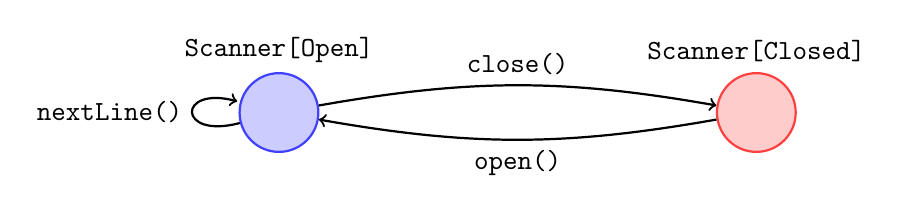
\begin{tikzpicture}
        \tikzstyle{open-file}=[circle, thick, draw=blue!75, fill=blue!20, minimum size=10mm]
        \tikzstyle{closed-file}=[circle, thick, draw=red!75, fill=red!20, minimum size=10mm]
        \tikzstyle{transition} = [->, thick];

        % \draw (0, 0) grid (\textwidth, 2);
        \node[open-file, label=above:\texttt{Scanner[Open]}] (open-file) at (0.25\textwidth, 1) {};
        \node[closed-file, label=above:\texttt{Scanner[Closed]}] (closed-file) at (0.75\textwidth, 1) {};
        \draw[transition]
            (open-file)
            edge[out=10, in=170] node[above] {\texttt{close()}}
            (closed-file) ;
        \draw[transition]
            (closed-file)
            edge[out=-170, in=-10] node[below] {\texttt{open()}}
            (open-file);
        \draw[transition]
            (open-file)
            edge[loop left] node {\texttt{nextLine()}}
            (open-file);
    \end{tikzpicture}
    \caption{The \texttt{Scanner} typestate state machine.}
    \label{fig:file-automata}
\end{figure}

\paragraph{What are typestates?}
In a nutshell, typestates can be thought as a mechanism to constrain APIs as the program state evolves.
More formally, typestates belong to the behavioral types category and
are built on the idea of lifting state to the type level since state becomes part of the type system,
the compiler should be able to reason about state,
effectively helping the developer track state and validate certain assumptions.

\paragraph{How are typestates useful?}
Diving deeper on how do typestates help the developer, we provide a simple yet classic example.
Consider a stream, whether it be a file or a socket, to be read, the stream must first be open before being read and finally closed.

\begin{code}
    \caption{\texttt{Scanner} misuse example.}
    \label{lst:scanner-misuse}
    \begin{minted}{java}
Scanner s = new Scanner(System.in); // open the stream
s.nextLine();                       // read
s.close();                          // close the stream
s.nextLine();                       // IllegalStateException
    \end{minted}
\end{code}

The code in \autoref{lst:scanner-misuse} tries to read a line after closing the stream,
it will crash during runtime with a \texttt{IllegalStateException} since you cannot read from a closed stream.

The fact that this code compiles without warnings (even when \texttt{-Xlint:all} is used) is problematic,
since the error will lead to a crash during runtime
(equally, if line 3 was \mintinline{java}{s = null;}, no warnings would issued).
While the presented example is simple, production-code is not,
and code paths that raise runtime errors may be untested until it reaches the hands of the user\footnote{\url{https://github.com/redis/jedis/issues/1747}}.

Using typestates solves the above problem by establishing a distinction between the open and closed \texttt{Scanner},
consider the code in \autoref{lst:typestated-scanner-usage}.

\begin{code}
    \caption{Typestated \texttt{Scanner} usage example.}
    \label{lst:typestated-scanner-usage}
    \begin{minted}{java}
Scanner[Open] s = new Scanner(System.in);   // open the stream
s.nextLine();                               // read
Scanner[Closed] s = s.close();              // close the stream
s.nextLine();                               // compile-time error
    \end{minted}
\end{code}

The compiler is now able to provide the developer with an error at compile-time
since it now knows that the \texttt{Scanner} is closed and thus,
it does not have a function \texttt{nextLine}.

\paragraph{Aliasing Control.}
Besides the pro-safety mentality of Rust,
another key detail which makes Rust a solid candidate for typestates is its aliasing control.

By definition, typestates are incompatible with aliasing
due to the fact that if an object is being used by $N$ clients,
when a client mutates an object, all other clients guarantees are broken.
Back to the stream example, if a client closes the stream,
all other clients may crash since they may try to read from a stream which is now closed.

While Rust is unable to enforce a truly linear type system (in which objects must be used \emph{exactly once}),
it is able to enforce an affine type system (or \emph{at most once} usage), as demonstrated in \autoref{lst:rust-move-semantics}.

% [3/1/2021]
% TODO [Add advantages to the linear//affine type system]

\begin{code}
    \caption{Rust move sematics example.}
    \label{lst:rust-move-semantics}
    \begin{minted}{rust}
let x = 0
let y = x;
println!("{}", x); // error, value moved in line 2
    \end{minted}
\end{code}

Such type system allows us to emulate typestates by \emph{forcing a move} whenever a state transition is required to happen,
this way, the previous state is “\emph{destroyed}” and cannot be mutated.

\subsection*{Typestating Rust}
Rust previously had a typestate system which was removed in version 0.4 since it “did not pull its own weight”.
The idea we propose is not aimed at bringing back the old typestate system but rather at leveraging Rust's type system to allow for typestated structures.
In short, we propose a DSL built with procedural macros which takes advantage of Rust's generics and affine type system capabilities.

\paragraph{The Typestate Pattern.}
As of now, it is possible for a developer to make use of typestates in Rust
the key idea is to write functions which consume the current object and return a new object
the function signature should be similar to \mintinline{rust}{fn transition(self: OldState, args...) -> NewState}.

Each state can then carry information, or not, being a simple 0-sized structure.
States can be grouped into sets using traits,
these sets can be further restricted using the sealed trait pattern\footnote{\url{https://git.io/JLbry}}.
An example implementation of the typestate pattern is available in \url{https://github.com/rustype/http-parser}.

% \begin{minted}{rust}
% trait StateTrait {}
% struct T<State: StateTrait> {
%     state: State
% }
% struct S1;
% impl StateTrait for S1 {}
% impl T<S1> {
%     fn transition(self) -> T<S2> {...}
% }
% struct S2;
% impl StateTrait for S2 {}
% impl T<S2> {
%     fn transition(self) -> Result<T<S2>> {...}
% }
% \end{minted}

\paragraph{Proposal.}
The code necessary to implement the typestate pattern requires a lot of boilerplate furthermore,
we want to be able to prove typestate properties (e.g. reachability and termination).
The former challenge can be solved through the use of macros, and the latter is not novel in the literature
to address it we just need to extract the state machine from the code and apply existing algorithms.

However, to do so without writing a static checker from the ground up we are required to use Rust's procedural function-like macros,
which enable the creation of a DSL for typestates,
thus solving both the boilerplate problem and the requirement for the ability to prove certain properties.

Existing work on the Rust ecosystem regarding typestate-like mechanisms is limited,
we have reviewed several automata crates and only one provided strong compile-time guarantees,
such crate was the \texttt{state\_machine\_future} crate,
however it requires a runtime such as Tokio due to being centered around asynchronous computations.

Our approach aims to extend the ideas behind \texttt{state\_machine\_future} with an expressive DSL and
the possibility to be used without a runtime in a purely static approach.
Currently, a prototype is under development and can be found in \url{https://github.com/rustype/typestate-rs}.

% \begin{minted}{rust}
% typestate! {
%     struct Drone {x: f32, y: f32}
%     fn ping_coords(&self) -> (f32, f32);
%     state Idle [last_landing: Time] {
%         transition take_off(self) -> Hovering;
%     }
%     state Hovering {
%         fn take_picture(&self, dst: &str);
%         transition land(self) -> Idle;
%     }
% }
% \end{minted}

\end{document}
